\chapter[$\ZZ$ Homology]{Simplicial $\ZZ$-Homology: Getting Oriented}
\section{Orientation and $\ZZ$-Homology}
\begin{note}
  We used $\msf H_n(K)$ to denote the $\zmod{2}$-homology gorups of a
  complex $K$. This was to simplify notation. In general, the notation
  is more like $\msf H_n(K; G)$, where $G$ is the group of
  coefficients for our module. When $G=\ZZ$, we drop the group and
  write $\msf H_n(K)$.
\end{note}

\begin{definition}[Edge orientation]
  For an edge $\set{vw}$, the two orientation classes correspond to
  two orderings of the vertices $v$ and $w$, and are denoted $\bk{vw}$
  and $\bk{wv}$. It is customary to think of the oriented edge
  $\bk{vw}$ as an edge with an arrow pointing from $v$ to $w$. We set
  $\bk{vw} = -\bk{wv}$.
\end{definition}
\begin{figure}[h]
  \centering
  \begin{tikzpicture}[
    decoration={
      markings,
      mark=at position 0.5 with {\arrow{>}}
    }]
    \node[draw, circle, fill=black, inner sep=1pt] (v1) at (-1,1) {};
    \node[above left] (v1l) at (v1) {$v$};
    \node[draw, circle, fill=black, inner sep=1pt] (w1) at (-1,-1) {};
    \node[below left] (w1l) at (w1) {$w$};
    \draw[thick, postaction={decorate}] (v1) -- (w1);

    \node[draw, circle, fill=black, inner sep=1pt] (v2) at (1,1) {};
    \node[above left] (v2l) at (v2) {$v$};
    \node[draw, circle, fill=black, inner sep=1pt] (w2) at (1,-1) {};
    \node[below left] (w2l) at (w2) {$w$};
    \draw[thick, postaction={decorate}] (w2) -- (v2);
  \end{tikzpicture}
  \caption{$\bk{vw}$ and $\bk{wv}$}
\end{figure}

\begin{definition}[Triangle orientation]
  For a triangle $\set{uvw}$ with vertices $u$, $v$, and $w$, the two
  orientation classes correspond geometrically to clockwise or
  counterclockwise orderings of the vertices when viewed a long a
  fixed normal.
\end{definition}

\begin{definition}[Oriented Simplex]
  Let $\simp{k}$ be a $k$-simplex, and let $\pi \in \mc S_n$. Then
  \[
    [v_0 \cdots v_k] = [v_{\pi(0)} \cdots v_{\pi(k)}]
  \]
  iff $\pi \in A_n$. If $\pi \not\in A_n$, we have
  \[
    [v_0 \cdots v_k] = -[v_{\pi(0)} \cdots v_{\pi(k)}]
  \]
  An $n$-simplex with a chosen orientation is called a \emph{Oriented
    simplex}. The boundary of a $0$-simplex is defined to be $0$.
\end{definition}

\begin{definition}[$n$-chain group]
  The $n$-\emph{chain group of $K$} is the free abelian group of
  oriented $K$-simplices under the equivalence relation above.
\end{definition}

\begin{definition}[Boundary map]
  For $n \geq 1$, the \emph{boundary of an oriented $n$-simplex}
  $\sigma = [v_0 \cdots v_n]$ is
  \[
    \partial(\sigma) = \sum_{i=0}^n (-1)^i \osimpdel{i}{n}
  \]
\end{definition}

\begin{problem}[18.3]
  For any $n$-simplex $\sigma$,
  \[
    \partial(-\sigma) = -\partial(\sigma)
  \]
\end{problem}
\begin{solution}
  Let $\sigma = \osimp{n}$. Since $(0\ 1)$ is odd, then
  \begin{align*}
    \osimp{n} = -\bk{v_1v_0\cdots v_n}
  \end{align*}
  hence
  \begin{align*}
    \partial(-\sigma)
    &= \partial(\bk{v_1v_0\cdots v_n}) \\
    &= \sum_{i=0}^n (-1)^i \osimpdel{i}{n} \\
    &= \bk{v_0v_2\cdots v_n} - \bk{v_1v_2 \cdots v_n} + \bk{v_1v_0v_3\cdots v_n} + \cdots + (-1)^n\bk{v_1v_0\cdots v_{n-1}} \\
    &= -\bk{v_1v_2\cdots v_n} + \bk{v_1v_2 \cdots v_n} - \bk{v_0v_1v_3\cdots v_n} + \cdots + (-1)^{n+1}\bk{v_0v_1\cdots v_{n-1}} \\
    &= \sum_{i=0}^n (-1)^{i+1} \osimpdel{i}{k} \\
    &= -\partial(\sigma)
  \end{align*}
  as desired.
\end{solution}
\begin{definition}[Boundary of an $n$-chain]
  The boundary of an $n$-chain is an $(n-1)$-chain given by
  \[
    \partial\pn{\sum_{i=1}^k c_i \sigma_i}
    = \sum_{i=1}^k c_i\partial(\sigma_i)
  \]
  Thus, the boundary is a homomorphism
  \[
    \partial_n : \msf C_n(K) \to \msf C_{n-1}(K)
  \]
\end{definition}
\begin{problem}[18.4]
  For all $n \geq 0$,
  \[
    \partial_n \circ \partial_{n+1}=0.
  \]
\end{problem}
\begin{solution}
  Let $\sigma \in \msf C_{n+1}(K)$ be given by
  \[
    \sigma = \sum_{i=0}^k c_i \sigma_i.
  \]
  Then
  \begin{align*}
    \partial_n \circ \partial_{n+1}(\sigma)
    &= \partial_n \pn{\sum_{i=0}^k c_i \partial_{n+1}(\sigma_i)} \\
    &= \pn{\sum_{i=0}^k c_i \partial_n \circ \partial_{n+1}(\sigma_i)}
    % \\
    % &= \sum_{i=0}^k c_i \partial_n\pn{\sum_{j=0}^{n+1} (-1)^j \osimpdel[v^{(i)}]{j}{n+1}} \\
    % &= \sum_{i=0}^k c_i
  \end{align*}
  hence it suffices to show that the claim holds on one of the $\sigma_i$. Note,
  \begin{align*}
    (\partial_n \circ \partial_{n+1})(\sigma_i)
    &= \partial_n\pn{\sum_{j=0}^{n+1} (-1)^j \osimpdel[v^{(i)}]{j}{n+1}} \\
    &= \sum_{j=0}^{n+1}\ \sum_{1 \leq \ell\neq j \leq n+1}^n (-1)^{j+\ell} \bk{v^{(i)}_0 \cdots \widehat{v^{(i)}_j} \cdots \widehat{v^{(i)}_\ell} \cdots v_{n+1}}
  \end{align*}
  conceivably, doing all the algebra out works.
\end{solution}
\begin{problem}[18.7]
  For a finite simplicial complex $K$, $\msf H_n(K)$ is a finitely
  generated abelian group.
\end{problem}
\begin{solution}
  Let $K$ be a finite simplicial complex. Then by definition, $\msf
  C_n(K)$ is finitely generated (by the two orientations of each of
  the $n$-simplices of $K$). Hence,
  \[
    \msf H_n(K) = \msf C_n(K)/\msf B_n(K)
  \]
  is finitely generated as well.
\end{solution}
\begin{problem}[18.8]
  If $K$ is simplicially connected, then $\msf H_0(K) \cong Z$. If $K$
  has $r$ connected components, then $\msf H_0(K)$ is a free abelian
  group of rank $r$.
\end{problem}
\begin{solution}
  Recall that $K$ is simplicially connected iff for all pairs of
  vertices $v_0, v_k$, there exists a sequence of 0-simplices
  $\set{v_i}_{1 \leq i \leq n}$ such that for all $1 \leq i \leq n-1$,
  $\set{v_iv_{i+1}}$ is a 1-simplex in $K$.

  Hence, for all 0-simplices $v_j, v_k \in K$, we have
  \[
    v_j \sim v_k
  \]
  by
  \[
    v_j - v_k = \partial\pn{\sum_{i=j}^{k-1} \set{v_iv_{i+1}}}.
  \]
  thus $\msf H_0(K)$ is a $\ZZ$-module with 1 basis element, so
  $H_0(K) \cong \ZZ$.

  Similarly, if $K$ has $r$ simplicially connected components, then
  $\msf H_0(K) \cong \ZZ^r$.
\end{solution}
\begin{problem}[18.9]
  If $K$ is a one-point space, $\msf H_n(K) \cong 0$ for $n > 0$, and
  $\msf H_0(K) \cong \ZZ$.
\end{problem}
\begin{solution}
  This follows directly as a corollary of the previous theorem.
\end{solution}

\section{Relative Simplicial Homology}
\begin{definition}[Relative Chain Group]
  Let $K'$ be a subcomplex of a simplicial complex $K$. Then the chain
  group $\msf C_n(K')$ can be viewed as a subgroup of the chain group
  $\msf C_n(K)$ consisting of all chains that are zero on any simplex
  outside $K'$. Then we can define the \emph{group of relative chains
    of $K$ modulo $K'$} as the quotient group
  \[
    C_n(K, K') = C_n(K)/C_n(K')
  \]
\end{definition}

% \begin{problem}[18.15]
%   Check that $\msf C_n(K,K')$ is a free abelian group.
% \end{problem}
% \begin{solution}

% \end{solution}
\begin{problem}[18.16]
  There is a boundary map
  \[
    \partial_n : \msf C_n(K, K') \to \msf C_{n-1}(K, K')
  \]
  such that $\partial_n \circ \partial_{n+1} = 0$ for all $n \geq 0$.
\end{problem}
\begin{solution}
  Let $\partial^{K}_n$ be the boundary map on $\msf C_n(K)$. Then
  define
  \[
    \partial_{n}(c_n)
    =
    \begin{cases}
      0 & \text{if } \partial^K(c_n) \in \msf C_{n-1}(K') \\
      \partial^K_n(c_n) & \text{otherwise }
    \end{cases}
  \]
  with linear extension.
\end{solution}

\begin{definition}[Relative Homology Group]
  As one might expect, we define
  \[
    \msf H_n(K, K')
    = \msf B_n(K, K') / \msf Z_n(K, K')
  \]
\end{definition}

\begin{problem}[18.25]
  The boundary map $\partial : \msf C_n(K) \to \msf C_{n-1}(K')$
  induces a well-defined map
  \[
    \partial : \msf H_n(K,K') \to \msf H_{n-1}(K').
  \]
\end{problem}
\begin{solution}
  Consider the following diagram:
  \begin{figure}[H]
    \centering
    \begin{tikzpicture}[scale=1.2]
      % \draw[help lines, color=gray!30, dashed] (-1.9,-1.9) grid (6,2);
      % \draw[->] (-2,0)--(6,0) node[right]{$x$};
      % \draw[->] (0,-2)--(0,2) node[above]{$y$};

      \foreach \n/\y/\h in {n+1/2.85/t, n/0/m, n-1/-2.85/b}{
        \node (0l\h) at (-5.5, \y) {$0$};
        \node (kp\h) at (-3, \y) {$\msf C_{\n}(K')$};
        \node (k\h) at (0, \y) {$\msf C_{\n}(K)$};
        \node (kkp\h) at (3, \y) {$\msf C_{\n}(K,K')$};
        \node (0r\h) at (5.5, \y) {$0$};
        \draw[->] (0l\h) -- (kp\h);
        \draw[->] (kp\h) -- (k\h) node[midway, above] {$i_{\n}$};
        \draw[->] (k\h) -- (kkp\h) node[midway, above] {$\pi_{\n}$};
        \draw[->] (kkp\h) -- (0r\h);
      }

      \foreach \ka/\kb/\n in {kpt/kpm/n+1, kpm/kpb/n, kt/km/n+1, km/kb/n, kkpt/kkpm/n+1, kkpm/kkpb/n}{
        \draw[->] (\ka) -- (\kb) node[midway, left] {$\partial_{\n}$};
      }

      \foreach \x in {-3,0,3}{
        \draw[->] (\x, 4.5) -- (\x, 3.2) node[midway, left] {$\partial_{n+2}$};
        \draw[->] (\x, -3.2) -- (\x, -4.5) node[midway, left] {$\partial_{n-1}$};
        \node (a) at (\x, 5) {$\vdots$};
        \node (a) at (\x, -5) {$\vdots$};
      }
    \end{tikzpicture}
    \caption{Diagram}
  \end{figure}
  we perform a diagram chase. Let ${\color{red} z_n} \in \msf
  Z_n(K,K') \subset \msf C_n(K,K')$. Then ${\color{red}\partial_n z_n}
  = 0\in \msf C_{n-1}(K,K')$. Further, since $\pi_n$ is surjective (by
  exactness), there exists $\color{green} c_n \in \msf C_n(K)$ such
  that $z_n = \pi_n(c_n)$.

  By the commutativity, of the diagram, $\partial_n \circ \pi_n (c_n)
  = \pi_{n-1} \circ \partial_n(c_n) = 0$. Thus, $\partial_n c_n \in
  \ker \pi_{n-1}$, so by exactness, $\partial_n c_n \in \im i_{n-1}$.
  Hence, there exists $c'_{n-1} \in \msf C_{n-1}(K')$ such that
  \[
    i_{n-1}(c'_{n-1}) = \partial_n c_n.
  \]
  We summarize the results so far in the following diagram:
  \begin{figure}[H]
    \centering
    \begin{tikzpicture}[scale=1.2]
      % \draw[help lines, color=gray!30, dashed] (-1.9,-1.9) grid (6,2);
      % \draw[->] (-2,0)--(6,0) node[right]{$x$};
      % \draw[->] (0,-2)--(0,2) node[above]{$y$};

      \foreach \n/\y/\h in {n+1/2.85/t, n/0/m, n-1/-2.85/b}{
        \node (0l\h) at (-5.5, \y) {$0$};
        \node (kp\h) at (-3, \y) {$\msf C_{\n}(K')$};
        \node (k\h) at (0, \y) {$\msf C_{\n}(K)$};
        \node (kkp\h) at (3, \y) {$\msf C_{\n}(K,K')$};
        \node (0r\h) at (5.5, \y) {$0$};
        \draw[->] (0l\h) -- (kp\h);
        \draw[->] (kp\h) -- (k\h) node[midway, above] {$i_{\n}$};
        \draw[->] (k\h) -- (kkp\h) node[midway, above] {$\pi_{\n}$};
        \draw[->] (kkp\h) -- (0r\h);
      }

      \foreach \ka/\kb/\n/\side in {kpt/kpm/n+1/left, kpm/kpb/n/left, kt/km/n+1/left, km/kb/n/left, kkpt/kkpm/n+1/right, kkpm/kkpb/n/right}{
        \draw[->] (\ka) -- (\kb) node[midway, \side] {$\partial_{\n}$};
      }

      \foreach \x in {-3,0,3}{
        \draw[->] (\x, 4.5) -- (\x, 3.2) node[midway, left] {$\partial_{n+2}$};
        \draw[->] (\x, -3.2) -- (\x, -4.5) node[midway, left] {$\partial_{n-1}$};
        \node (a) at (\x, 5) {$\vdots$};
        \node (a) at (\x, -5) {$\vdots$};
      }
      \node (zn) at (2.5, 2.4) {$\color{red} z_{n+1}$};
      \node (bzn) at (2.5, .6) {$0$};
      \draw[|->, red] (zn) -- (bzn) node[midway, left] {$\partial_{n+1}$};

      \node (cn) at (.5, 2.4) {$c_n$};
      \node[blue] (bcn) at (.5, .6) {$\partial_{n+1} c_n$};
      \draw[|->, red] (cn) -- (zn) node[midway, below] {$\pi_{n+1}$};
      \draw[|->, blue] (cn) -- (bcn) node[midway, right] {$\partial_{n+1}$};
      \draw[|->, blue] (bcn) -- (bzn) node[midway, above] {$\pi_{n}$};

      \node[black!30!green] (cn-1) at (-2.5, .6) {$c_{n}$};
      \filldraw[white] (-.2,.4) rectangle (.05,.8);
      \draw[black!30!green, |->] (cn-1) -- (bcn) node[midway, above] {$i_n$};
    \end{tikzpicture}
    \caption{Diagram}
  \end{figure}
  we now verify that $c_{n-1}$ is a cycle. Note that $\partial_n \circ
  \partial_{n+1}(c_n) = 0$. Since $i_{n-1}$ is injective, $\partial_n
  \circ \partial_{n+1}(c_n) = i_{n-1}(0)$. So by commutativity,
  \begin{figure}[H]
    \centering
    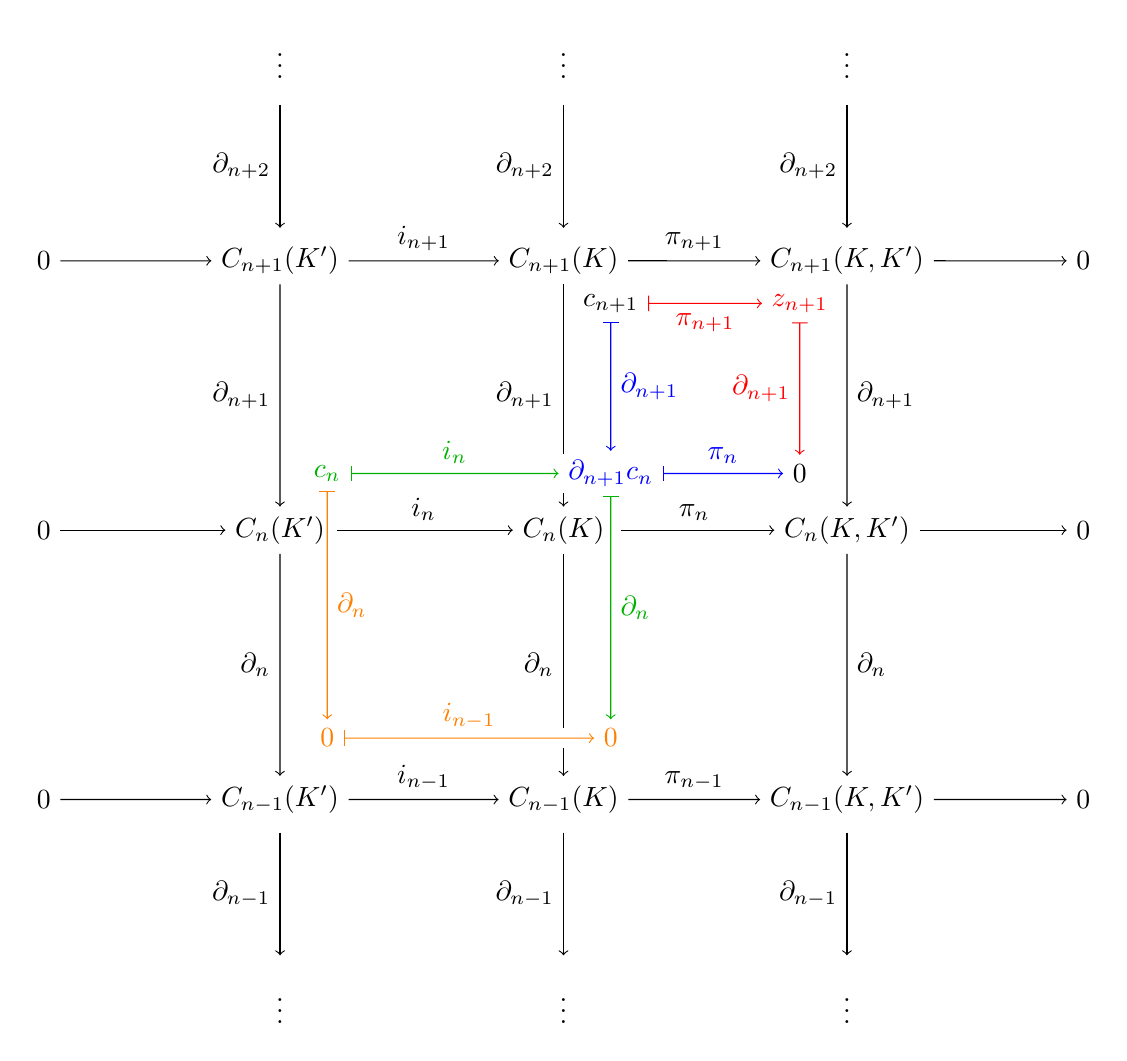
\begin{tikzpicture}[scale=1.2]
      % \draw[help lines, color=gray!30, dashed] (-1.9,-1.9) grid (6,2);
      % \draw[->] (-2,0)--(6,0) node[right]{$x$};
      % \draw[->] (0,-2)--(0,2) node[above]{$y$};

      \foreach \n/\y/\h in {n+1/2.85/t, n/0/m, n-1/-2.85/b}{
        \node (0l\h) at (-5.5, \y) {$0$};
        \node (kp\h) at (-3, \y) {$\msf C_{\n}(K')$};
        \node (k\h) at (0, \y) {$\msf C_{\n}(K)$};
        \node (kkp\h) at (3, \y) {$\msf C_{\n}(K,K')$};
        \node (0r\h) at (5.5, \y) {$0$};
        \draw[->] (0l\h) -- (kp\h);
        \draw[->] (kp\h) -- (k\h) node[midway, above] {$i_{\n}$};
        \draw[->] (k\h) -- (kkp\h) node[midway, above] {$\pi_{\n}$};
        \draw[->] (kkp\h) -- (0r\h);
      }

      \foreach \ka/\kb/\n/\side in {kpt/kpm/n+1/left, kpm/kpb/n/left, kt/km/n+1/left, km/kb/n/left, kkpt/kkpm/n+1/right, kkpm/kkpb/n/right}{
        \draw[->] (\ka) -- (\kb) node[midway, \side] {$\partial_{\n}$};
      }

      \foreach \x in {-3,0,3}{
        \draw[->] (\x, 4.5) -- (\x, 3.2) node[midway, left] {$\partial_{n+2}$};
        \draw[->] (\x, -3.2) -- (\x, -4.5) node[midway, left] {$\partial_{n-1}$};
        \node (a) at (\x, 5) {$\vdots$};
        \node (a) at (\x, -5) {$\vdots$};
      }
      \node (zn) at (2.5, 2.4) {$\color{red} z_{n+1}$};
      \node (bzn) at (2.5, .6) {$0$};
      \draw[|->, red] (zn) -- (bzn) node[midway, left] {$\partial_{n+1}$};

      \node (cn) at (.5, 2.4) {$c_{n+1}$};
      \node[blue] (bcn) at (.5, .6) {$\partial_{n+1} c_n$};
      \draw[|->, red] (cn) -- (zn) node[midway, below] {$\pi_{n+1}$};
      \draw[|->, blue] (cn) -- (bcn) node[midway, right] {$\partial_{n+1}$};
      \draw[|->, blue] (bcn) -- (bzn) node[midway, above] {$\pi_{n}$};

      \node[black!30!green] (cn-1) at (-2.5, .6) {$c_{n}$};
      \filldraw[white] (-.2,.4) rectangle (.05,.8);
      \draw[black!30!green, |->] (cn-1) -- (bcn) node[midway, above] {$i_n$};

      \filldraw[white] (-2.5, .05) rectangle (-2.4, -.05);
      \filldraw[white] (.5, .05) rectangle (.6, -.05);
      \filldraw[white] (-.05, -2.1) rectangle (.05, -2.3);

      \node[orange] (0b) at (.5, -2.2) {$0$};
      \node[orange] (0lb) at (-2.5, -2.2) {$0$};
      \draw[|->, black!30!green] (bcn) -- (0b) node[midway, right] {$\partial_n$};
      \draw[|->, orange] (cn-1) -- (0lb) node[midway, right] {$\partial_n$};
      \draw[|->, orange] (0lb) -- (0b) node[midway, above] {$i_{n-1}$};
    \end{tikzpicture}
    \caption{Diagram}
  \end{figure}
\end{solution}


%%% Local Variables:
%%% TeX-master: "../main"
%%% TeX-engine: default-shell-escape
%%% TeX-command-extra-option: -pdf
%%% End: